\documentclass[landscape]{foils}
\usepackage{fancybox}
\usepackage[pdftex]{geometry}
\geometry{headsep= 0.2in, footskip=0.2in, hscale=0.9}


\usepackage[pdftex]{color}  %for colors
                                            %   pdf effects
\usepackage[pdftex]{graphicx}     %for importing graphics
\usepackage{times}  %for nice fonts
\usepackage{pause} 
% for the colored background 
%\usepackage{background} 
%\usepackage{pp4slide} 
\usepackage{hyperref} %for hyperlinking and other 

\definecolor{DarkGreen}{rgb}{0.5,0.8,0.6}
\definecolor{RGBblack}{rgb}{0.0,0.0,0.0} 

\hypersetup{
  pdftitle={Presentation using \textsc{pdf}\LaTeX, \FoilTeX\, and \textsc{ppower4}},
  pdfsubject={How to make presentations with LaTeX},
  pdfauthor={Eugenia Yu and Weiliang Qiu,
    Department of Statistics,
    University of British Columbia},
  pdfkeywords={Presentations, LaTeX, FoilTeX, pdfTeX},
  pdfpagemode={FullScreen},                 %make the pdf start in full-screen
                                            %   mode
  %pdfpagemode={None},
  linkcolor=cyan,                           %make all the links cyan instead
  citecolor=cyan,                           %   of red
  pagecolor=blue,
  %pagecolor=cyan,
  urlcolor=cyan
  }


% the following four colors are the defaults for ppower4 slides
%\pagecolor{blue}                           %solid blue background
%\color{white}                              %for normal text
%\renewcommand\Black{\color{white}}         %for headers, etc.
%\renewcommand\normalcolor{\color{yellow}}  %for titles, etc.

% change the default background
%\hpagecolor[blue]{RGBblack}                %blue to black horizontal gradient
                                            %   background
%%%%\vpagecolor[blue]{RGBblack}                 %blue to black vertical gradient
                                            %   background


\leftheader{\textsc{Presentation using \textsc{pdf}\LaTeX, \FoilTeX\, and \textsc{ppower4}}}
                                            %make a left header
%\rightheader{\textsf{\thepage}}            %make a right header
\MyLogo{Eugenia and Weiliang, UBC Stats}    %make a left footer
%\rightfooter{}                             %make a right footer


\title{\shadowbox{Presentation using \textsc{pdf}\LaTeX, \FoilTeX\, and \textsc{ppower4}}} % the document title

% the author
\author{Latex Smart \\
         6356 Agricultural Road\\
         University of British Columbia\\
         Vancouver BC \\
         V6T 1Z2}

% the date
\date{\today}

\begin{document}

\thispagestyle{empty}

\setcounter{page}{0}

\maketitle

\foilhead{What is PPOWER4?}
\LogoOn
\textsc{ppower4} (\textsc{pdf} Presentation Post-Processor)
is a post-processor for \textsc{pdf} files produced
with \textsc{pdf}\LaTeX \, and \FoilTeX.

The features of PPower4:
\begin{itemize}
  \item 
 parts of a page can be
uncovered step by step during a presentation with {\tt Acrobat Reader}.
  \item can display parts of a page in any order
  \item can remove item from the page
  \item can insert fancy transitions or gradient background
\end{itemize}


\foilhead{Using PPower4}

Using \textsc{ppower4}:
\vspace{-0.2in}
\begin{itemize}
\item Add \verb|\usepackage{pause}|, \verb|\usepackage{background}|,\\
  \verb|\usepackage{pp4slide}|, \verb|\usepackage{hyperref}| to the
  preamble.
\item Produce \textsc{pdf} from \LaTeX \, source with
  \texttt{pdflatex file.tex}, then post-process with \texttt{ppower4
  file.pdf file.post.pdf}.  This produces a new file,
  \texttt{file.post.pdf}, with the effects. If you want to print out the pdf
file, {\bf print the orginal pdf file file.pdf} instead of the file
\texttt{file.post.pdf}.
\item Three different commands for backgrounds
  \begin{itemize}
  \item \verb|\pagecolor{color}| for solid color.
  \item \verb|\vpagecolor[color1]{color2}| for vertical gradient (like
    this page).
  \item \verb|\hpagecolor[color1]{color2}| for horizontal gradient.
  \end{itemize}
\end{itemize}

\foilhead{Using PPower4 (Ct'd)}

\begin{itemize}
\item The \verb|\pause| command produces partial pages.  For example
  at the end of this line there is a \verb|\pause| command\pause \,
  -- it waits for a keypress to display the rest of the page.
  \pauseDissolve  %Warning!  This is now the default transition for all
                  %   \pause commands and new pages.  It could get annoying!
  \begin{itemize}
  \item We can also use transition effects with \verb|\pause| like Dissolve
    or Wipe --- \verb+\pauseDissolve+ and \verb+\pauseWipe{0}+.
    \pauseWipe{0}  %Warning!  This is now the default transition for all
                   %   \pause commands and new pages.  It could get annoying!
                   %   The {0} is for direction, i.e. from the left.
  \item To Switch off the pause function, use \verb+\pauseReplace+.
  \end{itemize}
\end{itemize}

We can download the {\tt PPower4} program from the following site:

\href{http://www.tex.ac.uk/tex-archive/support/ppower4/download.html}{http://www.tex.ac.uk/tex-archive/support/ppower4/download.html}


\foilhead{Basics of Survival Analysis}
\LogoOff
\hypersetup{pdfpagetransition=Replace}
  Notations: \pause
  \begin{itemize}
    \item{ $T$ = a random variable representing time to event
           (e.g. time to death), $T > 0$ } \pauseDissolve
    \item{ pdf and cdf: $f(t)$ and $F(t)$ } \pause
    \item{ survivor function: $s(t)$ = $1-F(t)$ } \pauseVBlinds
    \item{ hazard function: $h(t)$, 
           which is the probability that an individual dies at
           time t, given that he has survived to time t.} \pause
    \item{ relationship between $h(t)$, $f(t)$, $s(t)$:\\
           $h(t)$ = $\frac{f(t)}{s(t)}$ \\
           $s(t)$ = exp$\{- \int^t_0 h(u) du \}$ \\
           So $f(t)$ = $h(t)$exp$\{- \int^t_0 h(u) du \}$
           } 
  \end{itemize}

\foilhead{Minipage and Graphics}
\LogoOn
\begin{minipage}[t]{4.5in}
  \raggedright
  \begin{center}
    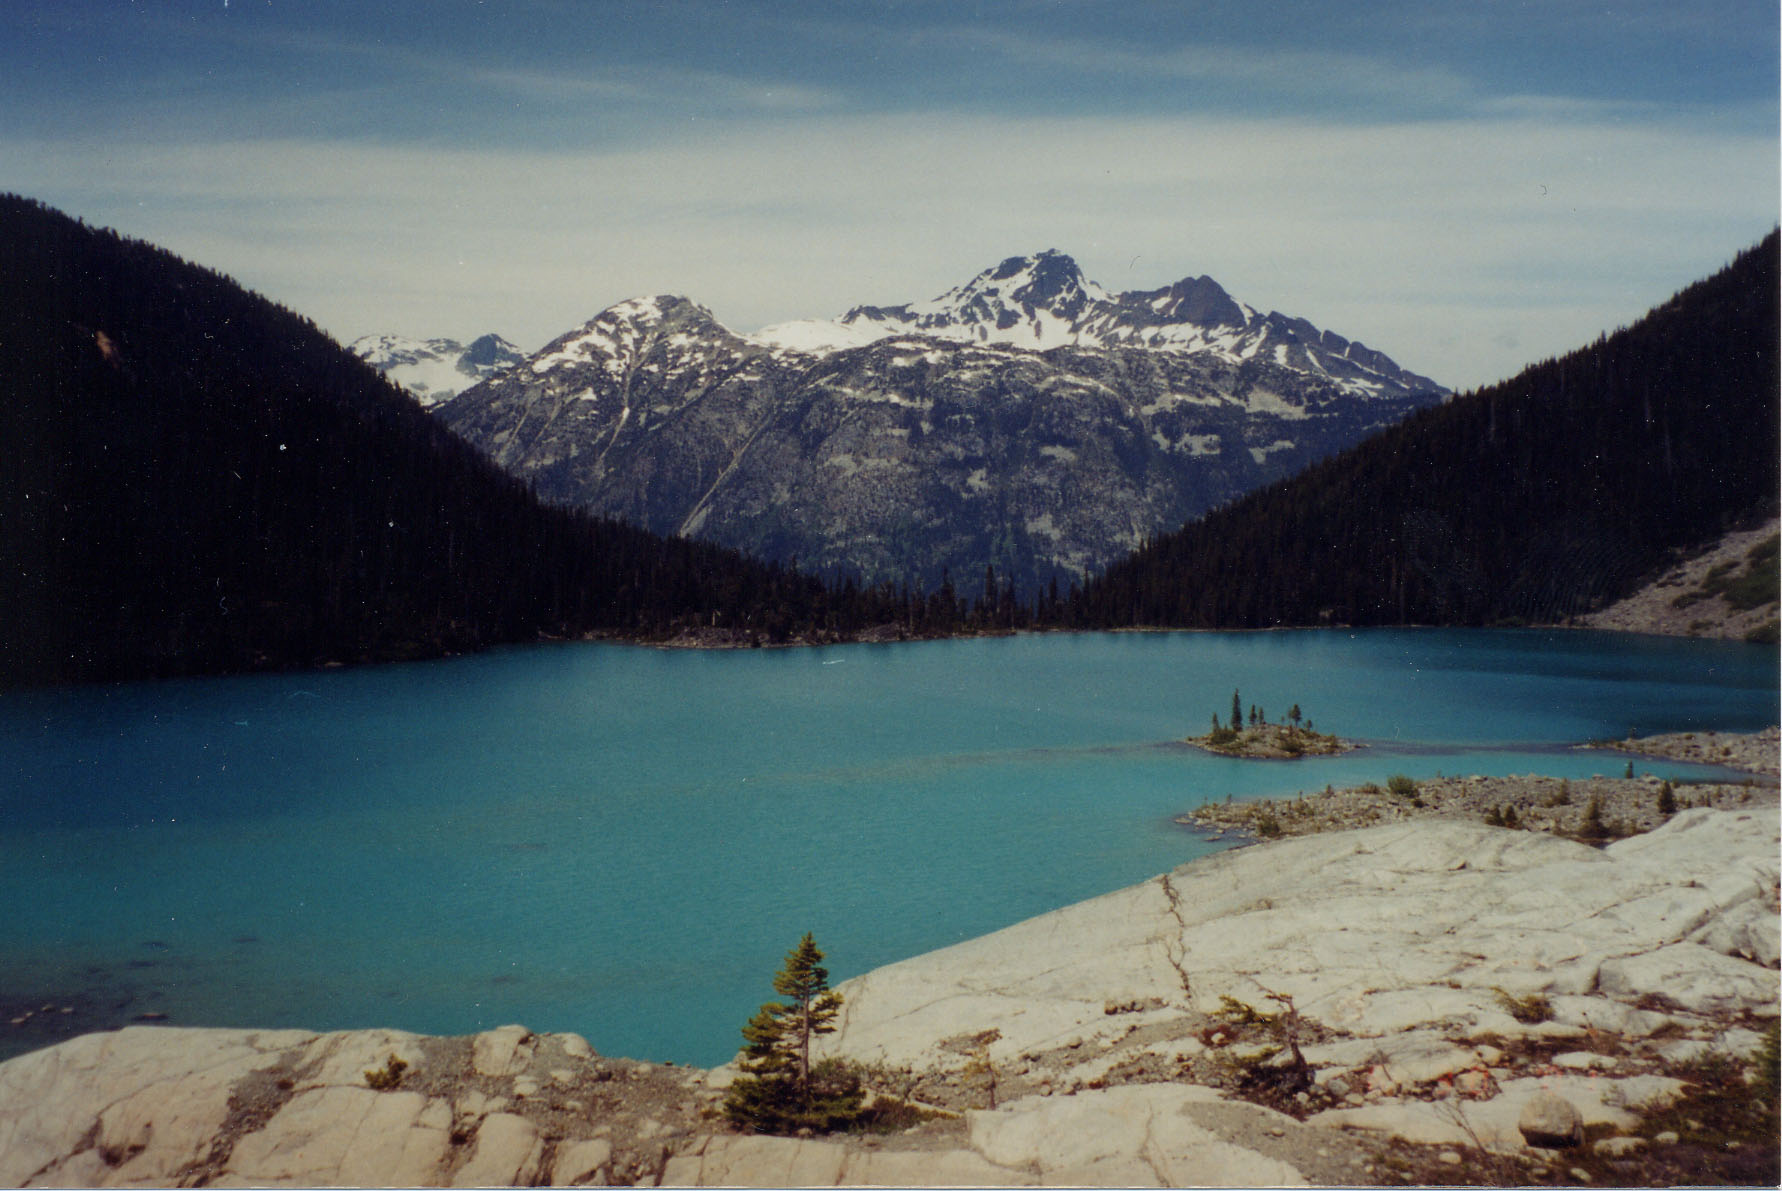
\includegraphics[width=2.8in,height=2in]{whistler}
  \end{center}
  \vspace{-0.2in}
  \begin{itemize}
  \item{\it Grad Trip}, August 2001 
  \vspace{-0.2in}
    \begin{itemize}
    \item Destination: Joffre Lake in Whistler \pauseHISplit
    \item People: UBC stats grads \pause 
    \item Activities: BBQ, hiking, canoeing, etc \pauseReplace
  \end{itemize}
 \end{itemize}
\end{minipage}
\hfill
\begin{minipage}[t]{4.5in}
  \raggedright
  \begin{center}
    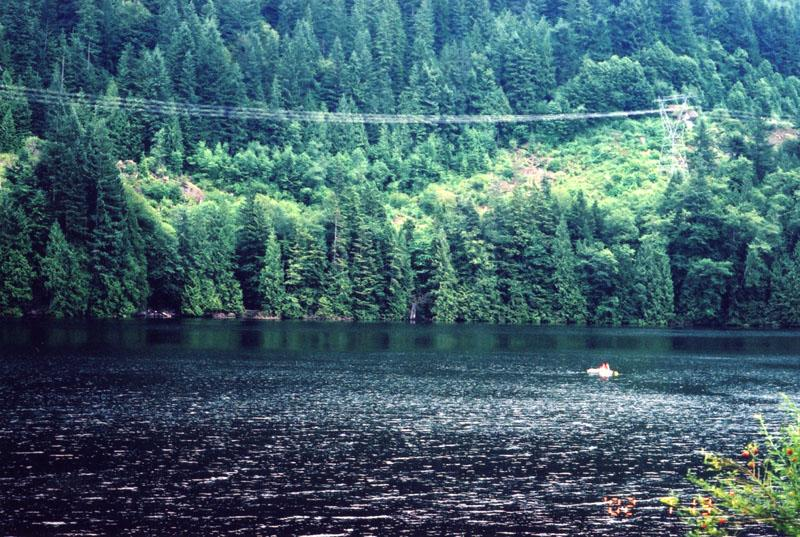
\includegraphics[width=2.8in,height=2in]{lake1}
  \end{center}
  \vspace{-0.2in}
  \begin{itemize}
  \item{\it Grad Trip}, July 2002 
  \vspace{-0.2in}
    \begin{itemize}
    \item Destination: Buntzen Lake in Port Moody 
    \item People: UBC and SFU stats grads 
    \item Activities: BBQ, hiking, kayaking, etc 
    \end{itemize}
  \end{itemize}
\end{minipage}

\foilhead{}
Partial code for the previous page:
\begin{verbatim}
\begin{minipage}[t]{4.5in}
  \raggedright
  \begin{center}
    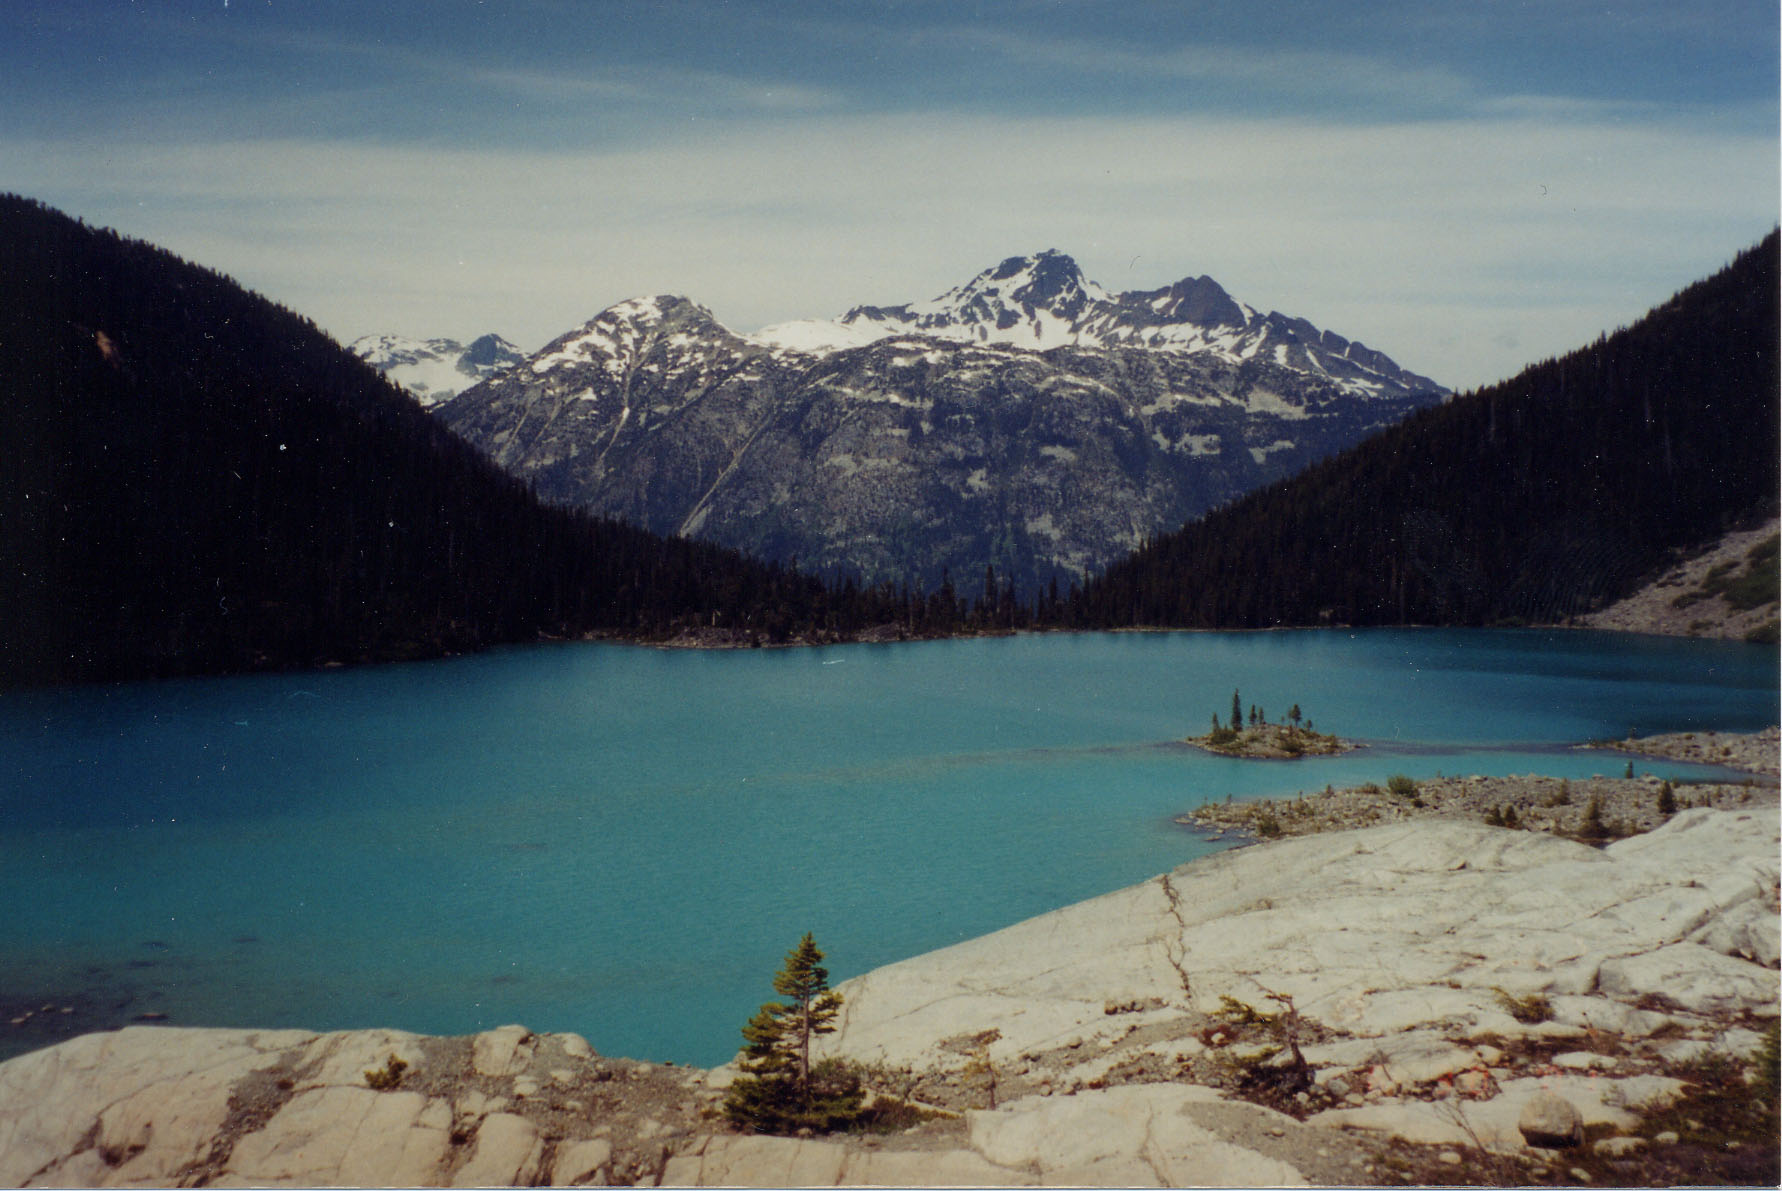
\includegraphics[width=2.8in,height=2in]{whistler}
  \end{center}
  \vspace{-0.2in}
  \begin{itemize}
  \end{itemize}
\end{minipage}
\hfill
\begin{minipage}[t]{4.5in}
\end{minipage}

\end{verbatim}


\end{document}
